\documentclass[11pt]{article}

% ---------- PACKAGES ----------
\usepackage[margin=1in]{geometry}
\usepackage{amsmath, amssymb, amsthm}
\usepackage{bm}
\usepackage{graphicx}
\usepackage{booktabs}
\usepackage{natbib}
\usepackage{hyperref}
\usepackage{algorithm,algpseudocode}
\usepackage{subcaption}
\hypersetup{
  colorlinks=true,
  linkcolor=blue,
  citecolor=blue,
  urlcolor=blue
}

% ---------- TITLE ----------
\title{1-Conformal predictive interval for right-censored survival data under finite observation window}
\author{}
\date{}

\begin{document}

\maketitle

\begin{abstract}
[placeholder]
\end{abstract}






\section{Setup}
We consider the construction of conformal predictive intervals for right-censored
survival data under a finite observation window.
Let $T$ denote the true event time and $\tau<\infty$ a fixed study horizon.
We define the truncated event time
\[
T^* = \min(T,\tau),
\]
which takes values in $[0,\tau]$ and represents the event time observable within
the follow-up window.
Our inferential target is a $(1-\alpha)$ predictive interval for $T^*$ given covariates:
for a new subject with covariate vector $z_0$, estimate
\[
\widehat C_{1-\alpha}(z_0)=\big[\widehat L_\alpha(z_0),\widehat U_\alpha(z_0)\big]
\]
such that the conformal marginal coverage criterion
\[
\Pr\!\left\{T^* \in \widehat C_{1-\alpha}(Z)\right\}\ge 1-\alpha
\]
is achieved approximately.

To capture both non-administrative and administrative censoring behavior, let $\widetilde C_i$ be a latent random censoring time and define the observed
censoring variable under finite horizon by
\[
C_i = \min(\widetilde C_i,\tau).
\]
Hence $C_i$ is a mixed random variable with a point mass at $\tau$.
Let $(Y_i,\Delta_i,Z_i)_{i=1}^n$ denote independent observations, where
\[
Y_i = \min(T_i, C_i) = \min(T_i^*, C_i), \qquad
\Delta_i = I(T_i \le C_i),
\]
and $Z_i \in \mathbb R^p$ is a vector of covariates.
We assume independent censoring,
$\widetilde C \perp (T,Z)$.

\section{Method}

Direct application of conformal inference is impeded by censoring.
Following the general strategy of resampling-based conformal calibration in \citet{qin_conformal_2025}, we approximate the joint distribution of $(T^*,Z)$ by a nonparametric estimator and generate synthetic samples for calibration.

\citet{qin_conformal_2025} define
\[
F_T(t,z)=\Pr(T\le t, Z\le z), \qquad G(t)=\Pr(C\ge t).
\]
In the original right-censored setting (targeting $(T,Z)$), the IPCW (inverse probability of censoring weighted) estimator
 takes the form
\[
\widehat F_T(t,z)=\frac{1}{n}\sum_{i=1}^n
\frac{\Delta_i I(Y_i\le t, Z_i\le z)}{\widehat G(Y_i^-)}.
\]

Now our target is the transformed variable $T^*=\min(T,\tau)$:
\[
F(t,z)=\Pr(T^*\le t, Z\le z), \qquad t\in[0,\tau].
\]
To derive a nonparametric estimator of this $F(t,z)$ on $(T^*,Z)$, we consider two cases.

\textbf{Case 1: $t<\tau$.}
\[
\begin{aligned}
F(t,z)
&=\Pr(\min(T,\tau)\le t,\ Z\le z) \\
&=\Pr(T\le t,\ Z\le z),
\end{aligned}
\]
because $\min(T,\tau)\le t<\tau$ implies $T\le t$.
So the estimator is the same IPCW form as for $F_T$.

\textbf{Case 2: $t=\tau$.}
\[
\begin{aligned}
F(\tau,z)
&=\Pr(\min(T,\tau)\le \tau,\ Z\le z) \\
&=\Pr(Z\le z) \\
&=\Pr(T\le \tau,\ Z\le z)+\Pr(T>\tau,\ Z\le z).
\end{aligned}
\]
Therefore, relative to the original $(T,Z)$ target, $F(\tau,z)$ has an extra
mass-at-$\tau$ component $\Pr(T>\tau,\ Z\le z)$.
Under $C=\min(\widetilde C,\tau)$, records with $(Y=\tau,\Delta=0)$ correspond to
this component, and it is estimated by reweighting with $G(\tau^-)$:
\[
\Pr(T>\tau,Z\le z)
=E\!\left[\frac{I(Y=\tau,\Delta=0,Z\le z)}{G(\tau^-)}\right].
\]
Hence, for $t<\tau$:
\[
\widehat F(t,z)
= \frac{1}{n} \sum_{i=1}^n
\frac{\Delta_i\, I(Y_i \le t, Z_i \le z)}{\widehat G(Y_i^-)}.
\]
And at $t=\tau$:
\[
\widehat F(\tau,z)
= \frac{1}{n} \sum_{i=1}^n
\frac{\Delta_i\, I(Y_i \le \tau, Z_i \le z)}{\widehat G(Y_i^-)}
+ \frac{1}{n} \sum_{i=1}^n
\frac{I(Y_i=\tau,\Delta_i=0,Z_i\le z)}{\widehat G(\tau^-)}.
\]
Equivalently, on $t\in[0,\tau]$,
\[
\widehat F(t,z)
= \frac{1}{n} \sum_{i=1}^n
\frac{\Delta_i\, I(Y_i \le t, Z_i \le z)}{\widehat G(Y_i^-)}
+ \frac{1}{n} \sum_{i=1}^n
\frac{I(Y_i=\tau,\Delta_i=0)\,I(t=\tau,\ Z_i\le z)}{\widehat G(\tau^-)}.
\]
where the first term estimates the continuous part from observed failures, and the
second term recovers the point mass at $T^*=\tau$. Because $C$ has mass at $\tau$,
we emphasize that $G(\tau^-)=\Pr(C\ge\tau)$ is used rather than $\Pr(C>\tau)$, to avoid a zero denominator in KM estimation implementation.

To construct the predictive interval, we adopt the Cox proportional hazards model
as a working model for $T^*$:
\[
\lambda(t \mid z) = \lambda_0(t)\exp(z^\top\beta), \qquad
S(t \mid z) = \exp\{-\Lambda_0(t)\exp(z^\top\beta)\},
\]
where $\Lambda_0(t)=\int_0^t \lambda_0(u)\,du$.
Define the monotone pivot
\[
U = S(T^* \mid Z),
\]
which is strictly decreasing in $T^*$ and therefore invertible.

\subsection{Algorithm}

\paragraph{Algorithm.}
\begin{enumerate}
\item Fit the Cox proportional hazards model on the observed data
to obtain estimators $\widehat\beta$ and $\widehat\Lambda_0(t)$.
\item Draw $B$ synthetic samples $(T^{*(b)}, Z^{(b)})$ i.i.d. from the estimated
joint distribution $\widehat F$.
\item For each draw, compute the pivot
\[
U^{(b)} = \exp\{-\widehat\Lambda_0(T^{*(b)})\exp(Z^{(b)\top}\widehat\beta)\}.
\]
\item Let $L$ and $R$ be the empirical $\alpha/2$ and $(1-\alpha/2)$ quantiles
of $\{U^{(b)}\}_{b=1}^B$.
\item For a new covariate value $z_0$, solve
\[
L \le \exp\{-\widehat\Lambda_0(t)\exp(z_0^\top\widehat\beta)\} \le R
\]
to obtain the predictive interval
\[
\widehat L_\alpha(z_0)
= \inf\{t:\exp[-\widehat\Lambda_0(t)\exp(z_0^\top\widehat\beta)] \le R\}, \quad
\widehat U_\alpha(z_0)
= \sup\{t:\exp[-\widehat\Lambda_0(t)\exp(z_0^\top\widehat\beta)] \ge L\}.
\]
The final interval is truncated to $[0,\tau]$.
\end{enumerate}

\begin{algorithm}[H]
\caption{Conformal Predictive Interval for $T^*$ under Finite Observation Window}
\label{alg:rcensored}
\begin{algorithmic}[1]

\Require Observed data $D=\{(Y_i,\Delta_i,Z_i)\}_{i=1}^n$, miscoverage level $\alpha$, calibration draws $B$, horizon $\tau$.
\Statex \textbf{Target:} $(1-\alpha)$ predictive interval for $T^*=\min(T,\tau)$.

\Procedure{ConformalPI}{$D,\alpha,B$}
    \State Fit Cox model to obtain $\widehat\beta$ and $\widehat\Lambda_0(t)$.
    \For{$b=1,\ldots,B$}
        \State Draw $(T^{*(b)},Z^{(b)}) \sim \widehat F$.
        \State Compute
        \[
        U^{(b)}=\exp\{-\widehat\Lambda_0(T^{*(b)})\exp(Z^{(b)\top}\widehat\beta)\}.
        \]
    \EndFor
    \State Let $(L,R)$ be the empirical $(\alpha/2,\ 1-\alpha/2)$ quantiles of $\{U^{(b)}\}_{b=1}^B$.
    \State \textbf{Output:} $(\widehat\Lambda_0,\widehat\beta,L,R)$.
\EndProcedure

\Statex
\Function{PredictTime}{$z_0$}
    \State Solve
    \[
    L \le \exp\{-\widehat\Lambda_0(t)\exp(z_0^\top\widehat\beta)\} \le R
    \]
    for $t \in [0,\tau]$.
    \State \textbf{Return:} predictive interval $[\widehat L_\alpha(z_0),\,\widehat U_\alpha(z_0)]$.
\EndFunction

\end{algorithmic}
\end{algorithm}

{\color{blue}
\paragraph{Remark (Lower bound for $T$).}
After obtaining the predictive interval
$[\widehat L_\alpha(z_0),\widehat U_\alpha(z_0)]$ for $T^*=\min(T,\tau)$, we also get
a one-sided lower bound for the original event time $T$.
Because $T\ge T^*$ almost surely, the event
$\{T^*\ge \widehat L_\alpha(Z)\}$ implies $\{T\ge \widehat L_\alpha(Z)\}$.
Also,
\[
\{\widehat L_\alpha(Z)\le T^*\le \widehat U_\alpha(Z)\}
\subseteq
\{T^*\ge \widehat L_\alpha(Z)\}.
\]
Hence
\[
\Pr\{T\ge \widehat L_\alpha(Z)\}
\ge
\Pr\{\widehat L_\alpha(Z)\le T^*\le \widehat U_\alpha(Z)\}
\ge 1-\alpha.
\]
So $\widehat L_\alpha(z_0)$ can be interpreted as a conservative lower prediction
bound for $T$.
}

{\color{blue}
\paragraph{Extension (Fixed-horizon risk).}
Besides outputting an interval for $T^*$, for a new unit with
covariate $z_0$ we want a single number at a fixed horizon $t_0\in[0,\tau]$
that summarizes ``risk by $t_0$'', which means the probability of event occurring before $t_0$. To estimate this probability,

Define
\[
u_0=\widehat S(t_0\mid z_0)
=\exp\{-\widehat\Lambda_0(t_0)\exp(z_0^\top\widehat\beta)\}.
\]
Using the same Monte Carlo draws from the main algorithm,
\[
U^{(b)}=\exp\{-\widehat\Lambda_0(T^{*(b)})\exp(Z^{(b)\top}\widehat\beta)\},
\qquad (T^{*(b)},Z^{(b)})\sim \widehat F,
\]
we define
\[
\widehat\pi_{\mathrm{marg}}(t_0,z_0)
=\frac1B\sum_{b=1}^B I\!\left\{U^{(b)}\ge u_0\right\}.
\]
This estimates
\[
\pi_{\mathrm{marg}}(t_0,z_0)
:=\Pr\!\left\{U\ge u_0\right\},
\qquad
U=\widehat S(T^*\mid Z),\ (T^*,Z)\sim \widehat F.
\]
So, consistent with the interval construction, $z_0$ enters through the
threshold $u_0$, while calibration is with respect to the estimated joint
distribution $\widehat F$. This is a marginally calibrated, $z_0$-adaptive probability, not a strictly conditional probability. For fixed $z_0$, since $u_0$
decreases as $t_0$ increases,
$\widehat\pi_{\mathrm{marg}}(t_0,z_0)$ is nondecreasing in $t_0$.
}






\section{Simulation study}



\subsection{Simulation design and sensitivity settings}
We evaluate the finite-window conformal predictive interval under a factorial simulation
design with one baseline scenario and three sensitivity axes:
(i) stronger covariate effects, (ii) higher Weibull shape, and
(iii) higher covariate dimension.
The event time is generated from a Weibull proportional hazards model:
\[
h(t\mid Z)=\frac{\gamma}{\kappa}\left(\frac{t}{\kappa}\right)^{\gamma-1}\exp(Z^\top\beta),\quad
T=\kappa\left\{\frac{-\log U}{\exp(Z^\top\beta)}\right\}^{1/\gamma},\ U\sim\mathrm{Unif}(0,1).
\]

For each replicate, we generate independent covariates $Z=(Z_1,\dots,Z_p)$ with
$Z_j\sim N(0,1)$, define $\tau$ as a fixed quantile of generated $T$, generate latent
censoring $\widetilde C\sim\mathrm{Exp}(\lambda_c)$, then set $C=\min(\widetilde C,\tau)$.
The observed data are $(Y,\Delta)$ with $Y=\min(T,C)$ and $\Delta=I(T\le C)$, and the
prediction target is $T^*=\min(T,\tau)$.

The rate $\lambda_c$ is calibrated to target approximately $10\%$, $20\%$, or $35\%$
non-administrative censoring before $\tau$. For each setting, we simulate $n=2000$
observations and split the data into training/testing subsets with proportion $70\%/30\%$.
The conformal method uses a Cox working model and Monte Carlo calibration with
$B=1500$ draws at $\alpha=0.1$. Each setting is repeated $30$ times, giving
$4\times 3\times 3=36$ settings and $1080$ total simulation replicates.

\begin{table}[htbp]
\centering
\caption{Simulation settings and sensitivity factors.}
\label{tab:sim_settings}
\begin{tabular}{@{}p{0.30\textwidth}p{0.64\textwidth}@{}}
\toprule
Component & Setting \\
\midrule
Failure-time DGP & Weibull PH with $\kappa=1$; shape $\gamma\in\{1.2,1.8\}$ (baseline $\gamma=1.2$). \\
Covariates & Independent normal covariates; baseline dimension $p=3$, high-dimension sensitivity $p=9$. \\
Regression effects & $\beta_j=0.30$ (baseline); stronger effect $\beta_j=0.60$. \\
Finite horizon $\tau$ & $\tau$ set to quantiles of generated $T$: $0.75$, $0.90$, $0.97$. \\
Censoring & $\widetilde C\sim\mathrm{Exp}(\lambda_c)$, $C=\min(\widetilde C,\tau)$, with target non-administrative censoring $10\%$, $20\%$, $35\%$. \\
Sample size and split & $n=2000$ per replicate; $70\%$ training and $30\%$ testing. \\
Conformal calibration & Cox working model; Monte Carlo draws $B=1500$; miscoverage $\alpha=0.1$. \\
Replicates & $30$ replicates per setting ($1080$ total). \\
\bottomrule
\end{tabular}
\end{table}

We report empirical coverage and mean interval length on the test set:
\[
\widehat{\mathrm{Cov}}=\frac{1}{n_{\text{test}}}\sum_{i=1}^{n_{\text{test}}}
I\!\left\{\widehat L_i\le T_i^*\le \widehat U_i\right\},\qquad
\widehat{\mathrm{Len}}=\frac{1}{n_{\text{test}}}\sum_{i=1}^{n_{\text{test}}}
(\widehat U_i-\widehat L_i).
\]

\subsection{Simulation results}
\begin{figure}[htbp]
\centering
\begin{subfigure}[t]{0.58\textwidth}
  \centering
  
\includegraphics[width=\linewidth]{Figures/direct_interval_coverage_examples.pdf}
  \caption{Empirical interval coverage examples.}
\end{subfigure}

\vspace{0.4em}
\begin{subfigure}[t]{0.58\textwidth}
  \centering
  
\includegraphics[width=\linewidth]{Figures/coverage_vs_tau.pdf}
  \caption{Coverage versus $\tau$ quantile.}
\end{subfigure}

\vspace{0.4em}
\begin{subfigure}[t]{0.48\textwidth}
  \centering
  
\includegraphics[width=\linewidth]{Figures/length_vs_tau.pdf}
  \caption{Mean interval length versus $\tau$ quantile.}
\end{subfigure}
\hfill
\begin{subfigure}[t]{0.48\textwidth}
  \centering
  
\includegraphics[width=\linewidth]{Figures/coverage_length_tradeoff.pdf}
  \caption{Coverage-length tradeoff.}
\end{subfigure}
\caption{Simulation results for finite-window conformal predictive intervals under
varying DGP, censoring targets, and $\tau$ settings. (a) Direct sample-level intervals
and coverage status. (b) Coverage versus $\tau$ quantile with nominal line and
replicate-level uncertainty bars. (c) Mean interval length versus $\tau$ quantile.
(d) Coverage-length tradeoff across settings.}
\label{fig:sim_results}
\end{figure}

Across all settings, the overall mean empirical coverage is $0.897$ for target $0.900$,
indicating good calibration under finite-window truncation.

Figure~\ref{fig:sim_results} presents the simulation results.
In panel (a), each horizontal line segment is one predicted interval
$[\widehat L_i,\widehat U_i]$ {\color{blue}for a randomly sampled subset (140 subjects) from the test set, ordered by estimated risk score $x^\top\widehat\beta$}, and the dot on that segment is the
corresponding true value $T_i^*$. Green means covered and orange means missed.
The vertical dashed line marks the realized $\tau$ in that facet, and each facet
corresponds to one $\tau$-quantile regime.
In panel (b), the $x$-axis is the $\tau$ quantile used in data generation and the
$y$-axis is mean empirical coverage; colors indicate censoring targets, error bars are
95\% CIs across replicates, and the dashed horizontal line is nominal coverage $0.9$.
In panel (c), the structure is the same as panel (b), but the $y$-axis is mean interval
length instead of coverage. In panel (d), each point is one simulation setting;
the $x$-axis is mean length, the $y$-axis is mean coverage, point color encodes
censoring target, and point shape encodes $\tau$ setting.

From the plots, panel (a) shows that most intervals cover their corresponding $T^*$,
and interval positions and widths shift as $\tau$ changes.
Panel (b) shows coverage remains close to nominal across the three $\tau$ regimes and
censoring targets, with only mild under-coverage in some high-censoring and large-$\tau$
settings. Panel (c) shows interval length increases as $\tau$ moves from the $0.75$
quantile to the $0.97$ quantile, which is expected because the range of $T^*$ becomes
wider. Panel (d) summarizes the coverage-length tradeoff: higher Weibull shape tends to shorten intervals, whereas strong signal and higher
dimension lead to longer intervals.

Averaging over censoring and $\tau$ settings, mean coverage is very similar across DGP
variants (baseline: $0.897$, strong signal: $0.898$, high shape: $0.897$,
high dimension: $0.896$). This indicates that empirical coverage is close to nominal and remains stable across different DGPs, while interval length differs more noticeably across parameter settings.

{\color{blue}
\subsection{Baseline comparison with a Cox plug-in interval}
To examine whether dropping conformal calibration yields narrower intervals, we add a
non-conformal benchmark that targets the same truncated event time
$T^*=\min(T,\tau)$. The benchmark fits the same Cox working model on the training
data, uses the fitted survival curve $\widehat S(t\mid z)$ to obtain the implied
predictive distribution of $T^*$, and then outputs the equal-tailed interval
\[
\big[\widehat Q_{T^*\mid z}(\alpha/2),\ \widehat Q_{T^*\mid z}(1-\alpha/2)\big]
\]
without conformal calibration.

For a fair comparison, we keep the baseline setting fixed:
$n=2000$, $p=3$, $\beta_j=0.30$, $\gamma=1.2$, $\kappa=1$,
$\tau$ at the $0.90$ quantile of $T$, target non-administrative censoring $0.20$,
$\alpha=0.10$, and the same $70\%/30\%$ train-test split.
The conformal method uses $B=1500$ Monte Carlo draws, while the Cox plug-in method
uses only the fitted Cox model. The comparison is repeated $20$ times.

\begin{figure}[htbp]
\centering
\begin{subfigure}[t]{0.95\textwidth}
  \centering
  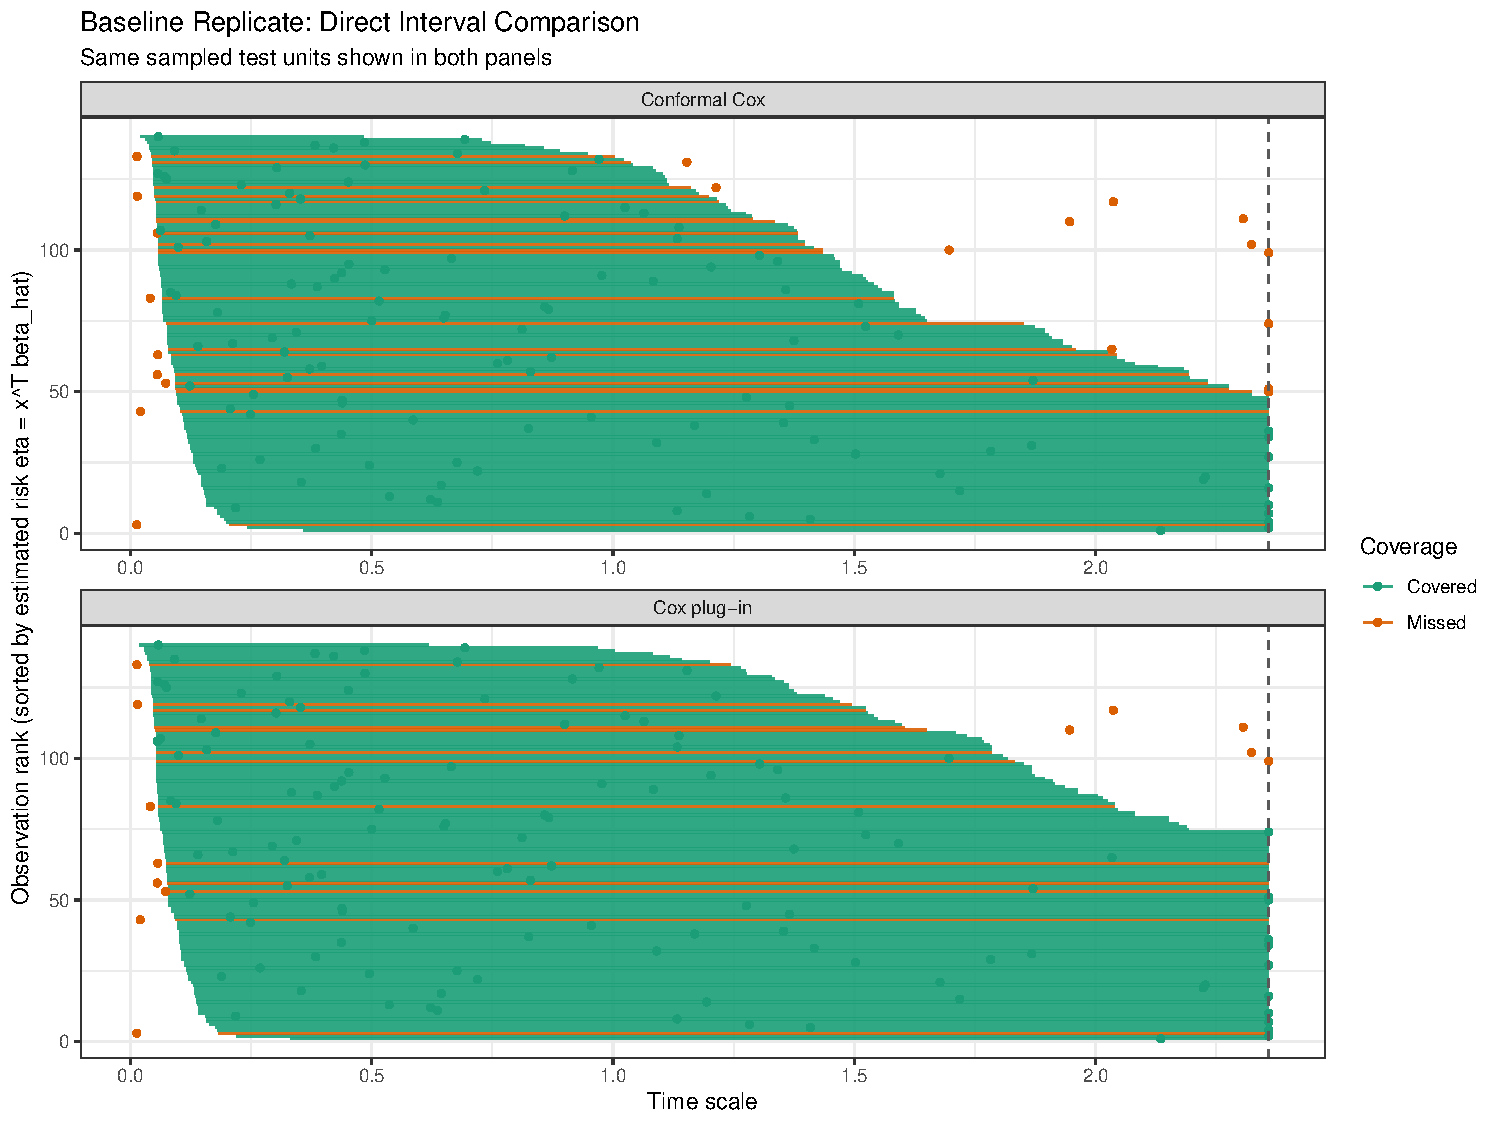
\includegraphics[width=\linewidth]{Figures/interval_examples_conformal_vs_cox_plugin.pdf}
  \caption{Direct comparison on the same $140$ sampled test units from one baseline replicate, ordered by $\eta=x^\top\widehat\beta$.}
\end{subfigure}

\vspace{0.4em}
\begin{subfigure}[t]{0.58\textwidth}
  \centering
  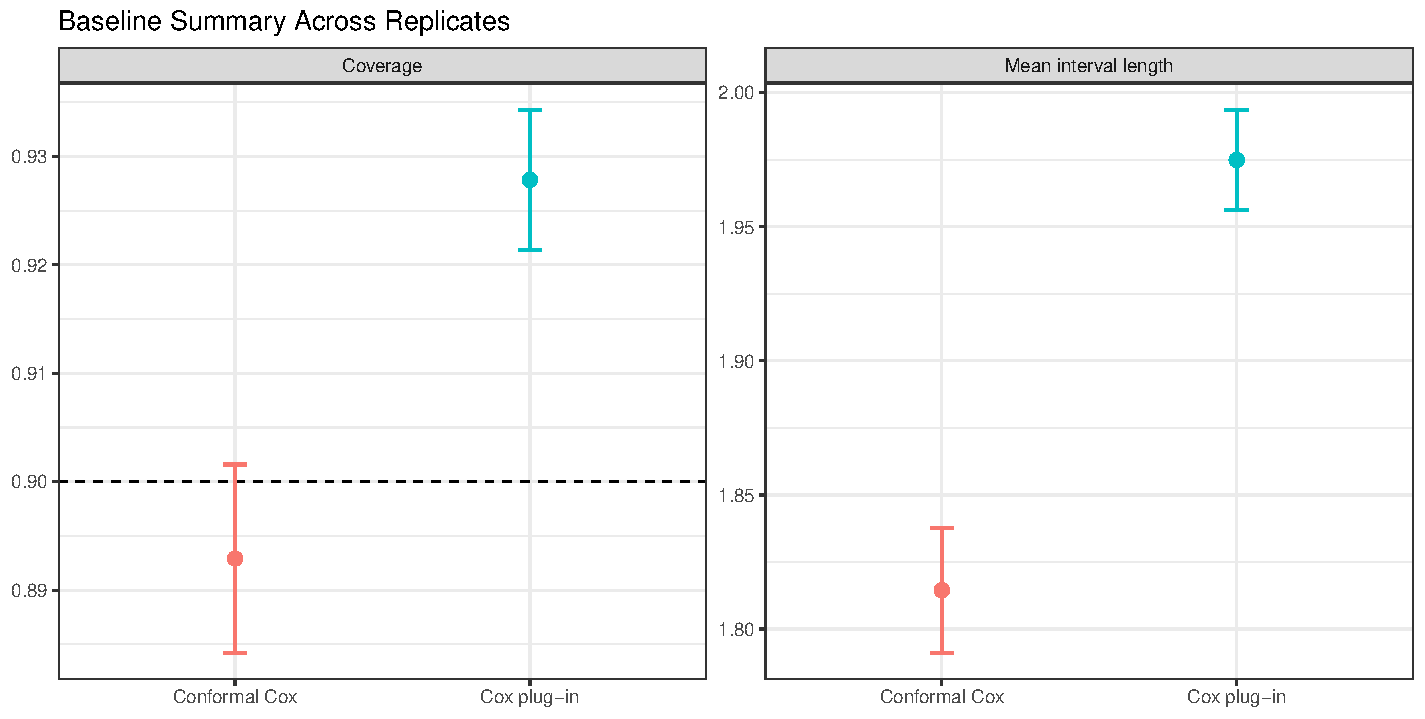
\includegraphics[width=\linewidth]{Figures/coverage_length_summary_by_method.pdf}
  \caption{Aggregate coverage and mean interval length across $20$ replicates.}
\end{subfigure}
\hfill
\begin{subfigure}[t]{0.36\textwidth}
  \centering
  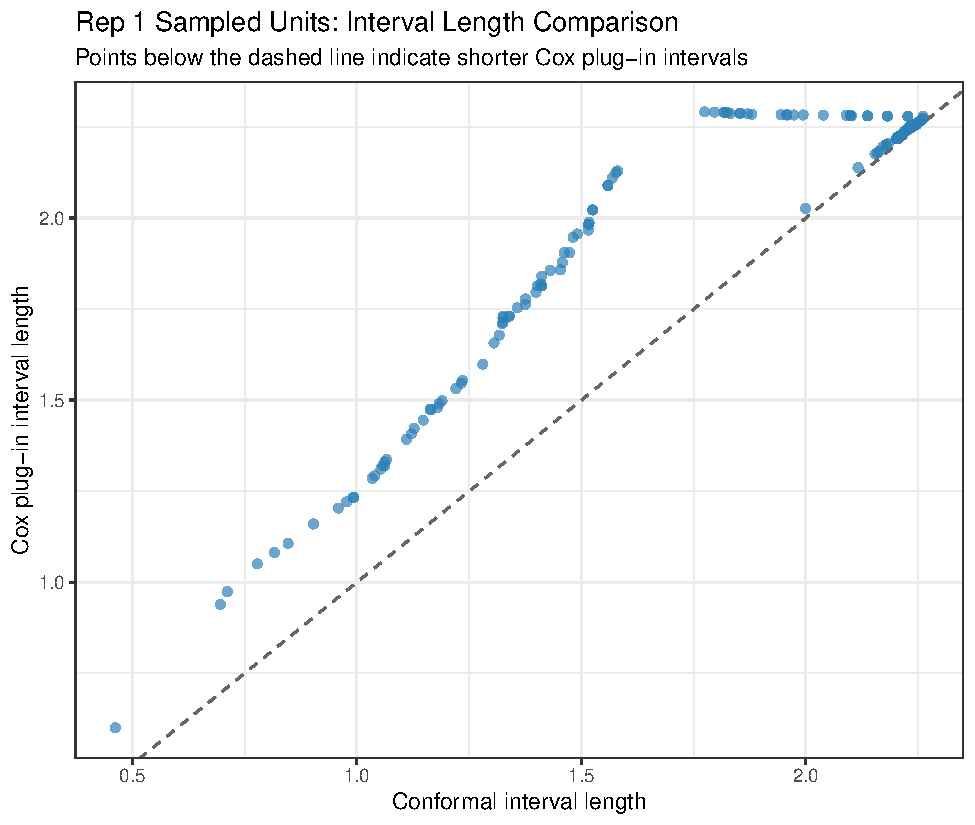
\includegraphics[width=\linewidth]{Figures/paired_length_scatter_rep1.pdf}
  \caption{Replicate-$1$ paired interval lengths for the same sampled units.}
\end{subfigure}
\caption{Baseline comparison between conformal Cox intervals and Cox plug-in intervals without conformal calibration. In panel (a), points are realized $T^*$ values and horizontal segments are predicted intervals under the two methods for the same sampled test subjects. In panel (b), points and error bars summarize replicate means and $95\%$ confidence intervals. In panel (c), points below the diagonal correspond to shorter Cox plug-in intervals.}
\label{fig:cox_plugin_compare}
\end{figure}

Figure~\ref{fig:cox_plugin_compare} shows that the Cox plug-in interval is not
narrower in this baseline setting. In panel (a), the plug-in intervals are often
slightly longer, especially near the upper end of the time axis. Panel (b) shows
the same pattern after aggregation: mean empirical coverage is about $0.893$ for the
conformal method and $0.928$ for the Cox plug-in benchmark, while mean interval
length is about $1.814$ and $1.975$, respectively. Panel (c) confirms this at the
sample level: most points lie above the diagonal, indicating longer Cox plug-in
intervals for the same test units. So, at least in this baseline experiment,
removing conformal calibration does not lead to tighter predictive intervals.
}




{\color{blue}
\subsection{Simulation for the fixed-horizon risk extension}
We additionally assess the extension in the baseline setting
($n=2000$, $p=3$, $\beta_j=0.30$, $\gamma=1.2$, $\kappa=1$,
$\tau$ at the $0.90$ quantile of $T$, censoring target $0.20$,
$\alpha=0.10$, $B=1500$).
Here $\eta:=x^\top\widehat\beta$ denotes the estimated linear predictor from the
working Cox model.
For one baseline replicate, we select four test units with different estimated
risk scores $x^\top\widehat\beta$ (approximately low to high), and compute
$\widehat\pi_{\mathrm{marg}}(t_0,z)$ on a grid of $t_0\in[0,\tau]$.

\begin{figure}[htbp]
\centering
\begin{subfigure}[t]{0.60\textwidth}
  \centering
  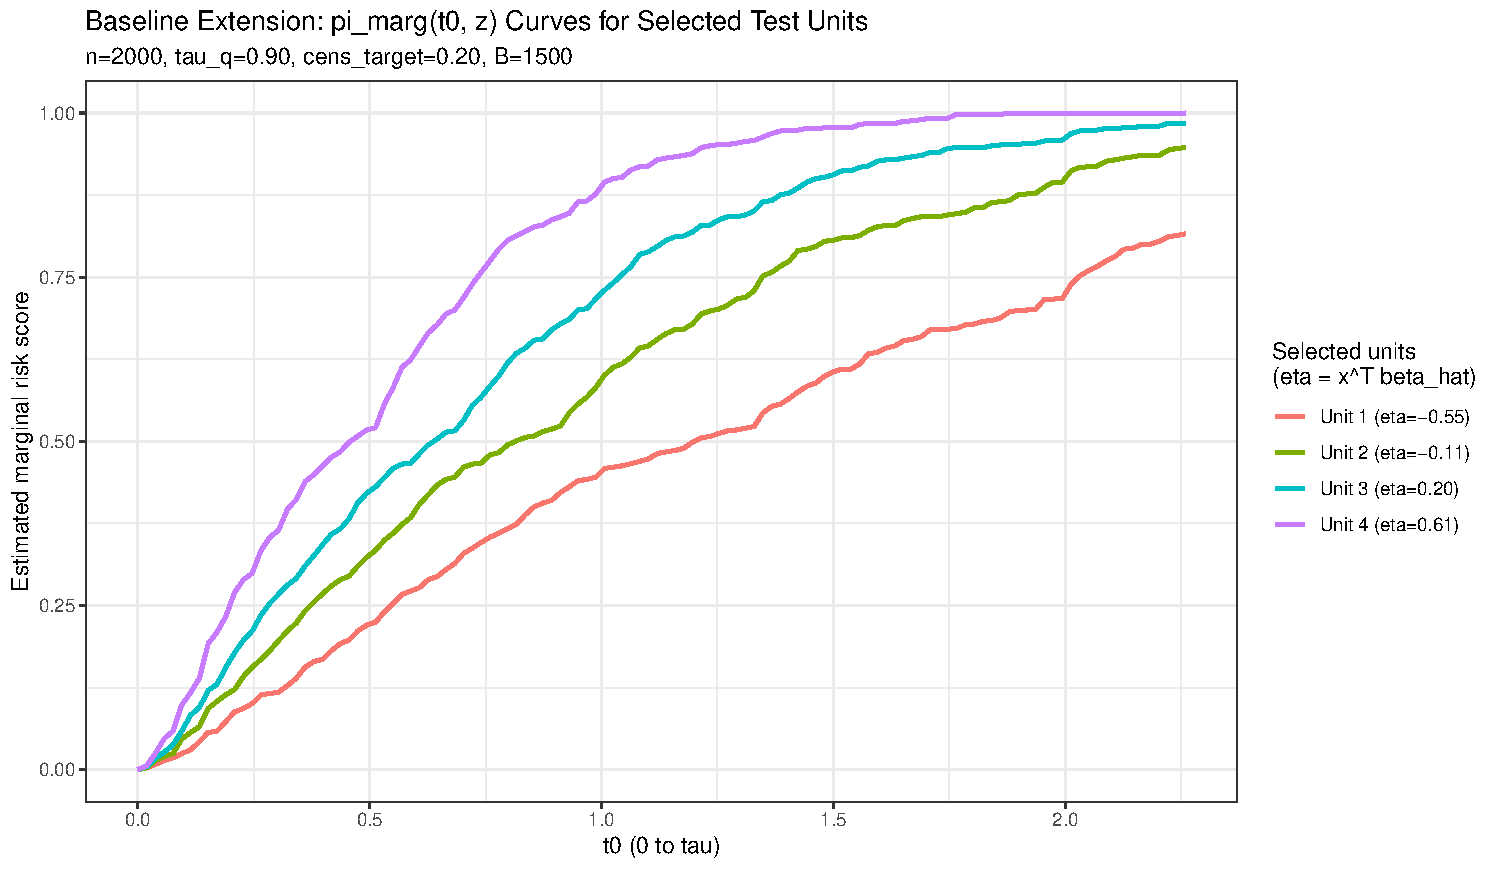
\includegraphics[width=\linewidth]{Figures/pi_vs_t0_selected_units.pdf}
  \caption{$\widehat\pi_{\mathrm{marg}}(t_0,z)$ curves for four selected test units.}
\end{subfigure}
\hfill
\begin{subfigure}[t]{0.37\textwidth}
  \centering
  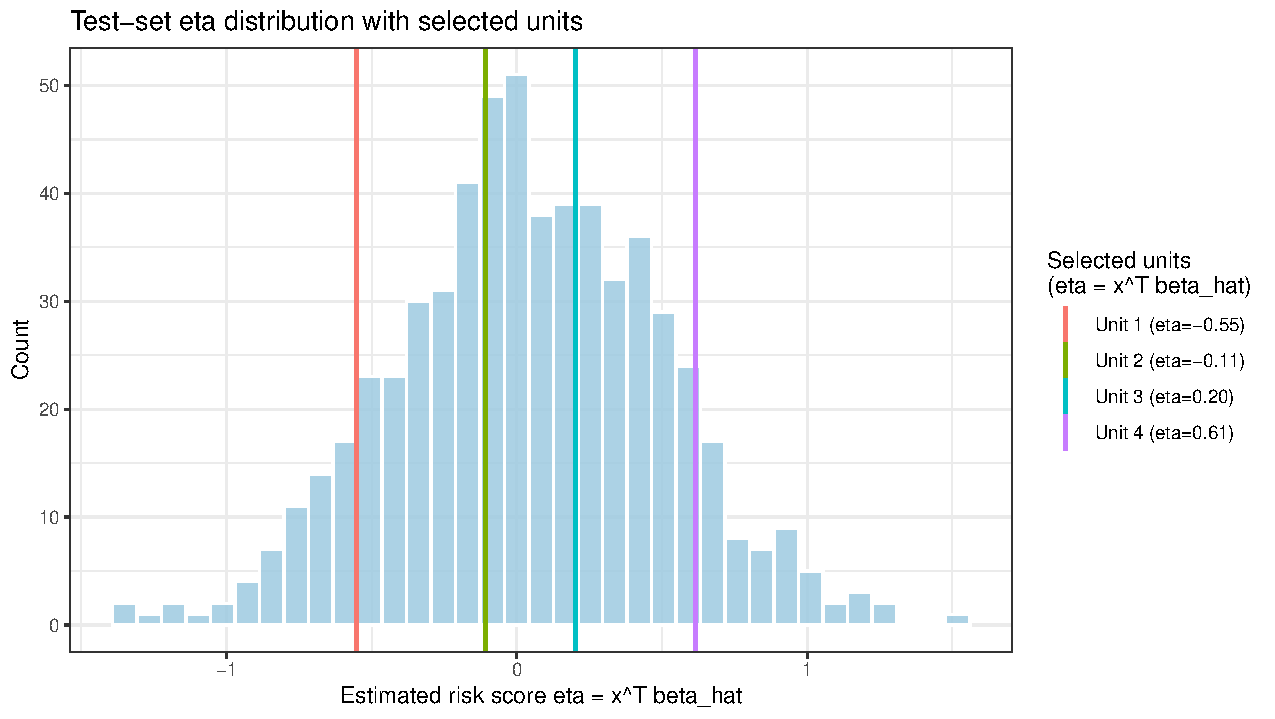
\includegraphics[width=\linewidth]{Figures/eta_distribution_selected_units.pdf}
  \caption{Test-set $\eta=x^\top\widehat\beta$ distribution and selected units.}
\end{subfigure}
\caption{Baseline simulation for the fixed-horizon risk-score extension.}
\label{fig:pi_extension}
\end{figure}

Figure~\ref{fig:pi_extension}(a) shows that, for each selected unit,
$\widehat\pi_{\mathrm{marg}}(t_0,z)$ increases with $t_0$, as expected.
Across units, the curves are ordered by risk level: units with larger
$x^\top\widehat\beta$ tend to have higher risk-score values at the same $t_0$.
Figure~\ref{fig:pi_extension}(b) provides a reference of the four samples with regard to $\eta=x^\top\widehat\beta$ distribution among the test set.
}

\bibliographystyle{apalike}
\bibliography{references}

\end{document}
